\chapter{Implementasi dan Pengujian}
\label{chap:implementasi_dan_pengujian}

Bab ini terdiri atas implementasi, pengujian, dan masalah yang dihadapi. Pada bagian implementasi dijelaskan mengenai lingkungan implementasi dan hasil dari implementasi. Pada bagian pengujian berisi hasil dari pengujian. Pada bagian masalah yang dihadapi dijelaskan masalah-masalah yang dihadapi pada saat implementasi.

\section{Implementasi}
\label{sec:implementasi}

\subsection{Lingkungan Implementasi}
\label{ssec:lingkungan_implementasi_dan_pengujian}

Berikut adalah spesifikasi \textit{laptop} yang digunakan untuk implementasi:
\begin{enumerate}
    \item \textit{Processor} : Intel Core i3-4030U 1.9 Ghz
    \item \textit{Memory} : 6144MB Ram
    \item \textit{Storage} : 500GB HDD dan 250GB SSD
    \item \textit{VGA} : NVDIA GeForce 840M + Intel HD Graphics Family
    \item \textit{Operating System} : Windows 10 64-bit\\
\end{enumerate}

Berikut adalah spesifikasi perangkat lunak yang digunakan untuk implementasi:
\begin{enumerate}
    \item IDE : Eclipse IDE Photon Release (4.8.0)
    \item Bahasa Pemrograman : Java
    \item \textit{Java Library} : Java 1.8.0\_181\\
\end{enumerate}

Berikut adalah spesifikasi node sensor yang digunakan untuk implementasi:
\begin{enumerate}
    \item Nama : Preon32
    \item \textit{Processor} : Cortex-M3
    \item \textit{Operating System} : PreonVM
    \item Penyimpanan Sistem : 64 kByte SRAM
    \item Penyimpanan Data : 256 kByte Flash
    \item Pita frekuensi : 2400.0 - 2483.5 MHz
    \item Jangkauan : 250 meter (luar ruangan) dan 30 meter (dalam ruangan)
    \item Sensor-sensor : Sensor suhu, sensor cahaya, sensor kelembaban, sensor tekanan udara, dan sensor getaran.
\end{enumerate}

\subsection{Hasil Implementasi}

Hasil Implementasi ini adalah aplikasi sesuai dengan perancangan pada Bab \ref{chap:perancangan}. Implementasi aplikasi ini menggunakan Bahasa Pemrograman Java. Terdapat kelas-kelas yang akan diunggah ke dalam node sensor yaitu kelas BS dan kelas NS. Selain kelas-kelas yang diunggah ke dalam node sensor, terdapat juga kelas yang akan menghubungan \textit{base station} dengan komputer pengguna menggunakan \textit{command line interface} yaitu kelas Handler. Untuk mendapatkan data diperlukan juga kelas-kelas untuk menangani setiap sensor pada Preon32.

\subsubsection{Kelas AccelerationSensor}
Kode program kelas ini dapat dilihat pada Lampiran \ref{lamp:A} listing \ref{accl}. Pada kelas ini terdapat metode \textit{run}. Di dalam metode \textit{run} terdapat variabel lokal \textit{spi} dengan tipe NativeSPI yang berfungsi untuk \textit{driver bus}. Sebelum dapat melakukan \textit{sensing}, harus dinyalakan dahulu driver NativeSPI dan GPIO. Nilai yang didapat dari sensor ini terdiri dari 3 nilai dan disimpan ke dalam variabel \textit{values}. Nilai \textit{values} ini kemudian akan disimpan ke dalam atribut \textit{temp} dengan format "A: [x,y,z]". Pada kelas ini juga terdapat metode \textit{getTemp} untuk mengembalikan nilai dari atribut \textit{temp}. 

\subsubsection{Kelas HumiditySensor}
Kode program kelas ini dapat dilihat pada Lampiran \ref{lamp:A} listing \ref{humid}. Pada kelas ini terdapat metode \textit{run} yang menyalakan driver SHT21 tersebut dan membuat format "H: + rh" dan disimpan ke dalam atribut \textit{temp}. Pada kelas ini juga terdapat metode \textit{getTemp} yang berfungsi untuk mengembalikan nilai dari atribut \textit{temp}.

\subsubsection{Kelas TemperatureSensor}
Kode program untuk kelas ini dapat dilihat pada Lampiran \ref{lamp:A} listing \ref{temp}. Pada kelas ini terdapat metode \textit{run}. Pada metode \textit{run}, driver untuk sensor suhu tersebut dinyalakan. Suhu yang didapat adalah suhu dalam celsius dan disimpan ke dalam variabel lokal \textit{celsius}. Kemudian atribut \textit{temp} akan diisi dengan format "T: + celsius + [C]". Pada kelas ini juga terdapat metode \textit{getTemp} yang mengembalikan nilai dari atribut \textit{temp}.

\subsubsection{Kelas sensing}
Kode program kelas ini dapat dilihat pada Lampiran \ref{lamp:A} listing \ref{sensing_class}. Kelas ini digunakan untuk menggabungkan ketiga sensor yang digunakan menjadi sebuah string. String ini yang akan disimpan nantinya ke dalam file. Terdapat metode \textit{sense} dengan tipe String yang mengembalikan nilai gabungan dari ketiga sensor tersebut. Pertama-tama harus dinyalakan dahulu driver \textit{NativeI2C}. Kemudian memanggil metode \textit{run} dari setiap objek sensor yang telah dibuat. Metode \textit{sense} akan mengembalikan String.

\subsubsection{Kelas BS}
Kode program kelas ini dapat dilihat pada Lampiran \ref{lamp:A} listing \ref{BS}. Saat dijalankan, kelas ini akan menginisialisasi atribut-atribut yang digunakan seperti menginisialisasi \textit{hmapSN} dengan \textit{key} adalah semua node pada \textit{node\_list}, dan \textit{value} 1. Setelah itu akan dipanggil metode \textit{startUSART}. Metode \textit{startUSART} ini digunakan untuk melakukan inisialisasi USART yang digunakan untuk mengirim pesan kepada komputer pengguna. Setelah itu akan dipanggil metode \textit{runs}. 

Metode \textit{runs} digunakan untuk mengaktifkan radio, \textit{tranceiver}, dan membuat objek \textit{FrameIO}. Di dalam metode ini juga akan dipanggil metode \textit{sender} dan \textit{receiver} di dalam sebuah \textit{thread} yang terus berjalan.

Metode \textit{sender} digunakan untuk mengirimkan perintah kepada semua node ADDR\_NODE2. Pesan ini bergantung pada masukan pengguna melalui program pengguna (Handler). Pada metode ini menggunakan USART untuk menerima pesan tersebut. Jika masukan tersebut adalah '0', maka yang dikirim adalah pesan "EXIT". Jika  masukan tersebut adalah '1', maka yang dikirim adalah pesan "ON". Jika masukan tersebut adalah '2', maka yang dikirim adalah pesan "Q" + Waktu saat ini sesuai dengan waktu komputer pengguna. Jika masukan tersebut adalah '3', maka pesan yang dikirim adalah pesan "WAKTU". Jika masukan tersebut adalah '4', maka pesan yang dikirim adalah pesan "DETECT". Implementasi dari metode \textit{sender} dapat dilihat pada listing \ref{sender_bs}

\begin{lstlisting}[label=sender_bs, language=Java, caption=Metode sender pada kelas BS, numbers=none]
    public static void sender(final FrameIO fio) throws Exception {
		new Thread() {
			public void run() {
				while (true) {
					int temp = 0;
					try {
						temp = usart.read();
					} catch (USARTException e1) {
						e1.printStackTrace();
					}
					if (temp == 0) {
						try {
							for (int i = 0; i < ADDR_NODE2.length; i++) {
								send("EXIT", ADDR_NODE2[i], fio);
							}
						} catch (Exception e1) {
							e1.printStackTrace();
						}
						exit = true;
						firstSense = false;

						break;
					} else if (temp == 1) {
						try {
							for (int i = 0; i < ADDR_NODE2.length; i++) {
								send("ON", ADDR_NODE2[i], fio);
							}
						} catch (Exception e1) {
							e1.printStackTrace();
						}
					} else if (temp == 2) {
						long currTime = Time.currentTimeMillis();
						try {
							for (int i = 0; i < ADDR_NODE2.length; i++) {
								send(("Q" + currTime), ADDR_NODE2[i], fio);
							}
						} catch (Exception e1) {
							e1.printStackTrace();
						}
					} else if (temp == 3) {
						try {
							for (int i = 0; i < ADDR_NODE2.length; i++) {
								send("WAKTU", ADDR_NODE2[i], fio);
							}
						} catch (Exception e1) {
							e1.printStackTrace();
						}
					} else if (temp == 4) {
						firstSense = true;
						try {
							for (int i = 0; i < ADDR_NODE2.length; i++) {
								send("DETECT", ADDR_NODE2[i], fio);
							}
						} catch (Exception e1) {
							e1.printStackTrace();
						}
					}
				}
			}
		}.start();
	}
\end{lstlisting}

Metode \textit{receiver} digunakan untuk menerima \textit{Frame} dari node ADDR\_NODE2. \textit{Frame} tersebut berisi pesan atau \textit{payload}. Jika pesan diakhiri dengan huruf 'E' atau diawali dengan huruf 'T' maka pesan tersebut akan ditambahkan dengan awalan dan akhiran '\#' kemudian dikirimkan melalui USART. 

Jika pesan yang diterima diawali dengan kata "SENSE" berarti pesan tersebut adalah data hasil \textit{sensing}. Disini pesan tersebut akan dipecah untuk mendapatkan alamat utama node pengirim pesan, dan \textit{sequence number}. Untuk menghindari duplikasi harus dilakukan pengecekan \textit{sequence number} tersebut. Setelah itu \textit{base station} akan mengirimkan ACK kepada alamat yang terdapat pada \textit{frame} tersebut.
Implementasi dari metode \textit{receiver} dapat dilihat pada listing \ref{receiver_bs}
\begin{lstlisting}[label=receiver_bs, language=Java, caption=Metode receiver pada kelas BS, numbers=none]
    public static void receive(final FrameIO fio) throws Exception {
		Thread receive = new Thread() {
			public void run() {
				Frame frame = new Frame();
				while (true) {
					try {
						fio.receive(frame);
						byte[] dg = frame.getPayload();
						String str = new String(dg, 0, dg.length);						
						if (str.charAt(str.length() - 1) == 'E') {
							String msg = "#" + str + "#";
							try {
								out.write(msg.getBytes(), 0, msg.length());
								usart.flush();
							} catch (Exception e) {
								e.printStackTrace();
							}
						}
						else if (str.charAt(0) == 'T') {
							String msg = "#" + str + "#";
							try {
								out.write(msg.getBytes(), 0, msg.length());
								usart.flush();
							} catch (Exception e) {
								e.printStackTrace();
							}
						} else if (str.startsWith("SENSE")) {
							int beginNode = str.indexOf('<');
							int beginSN = str.indexOf('>');
							int endSN = str.indexOf('?');
							int node = Integer.parseInt(str.substring(beginNode + 1, beginSN));
							int sn = Integer.parseInt(str.substring(beginSN + 1, endSN));
							if (hmapSN.get(node) == sn) {
								String msg = "#" + str + "#";
								try {
								out.write(msg.getBytes(), 0, msg.length());
									usart.flush();
									Thread.sleep(50);
								} catch (Exception e) {
									e.printStackTrace();
								}
								hmapSN.put(node, sn+1);
							}
							send("ACK" + node+"."+sn, frame.getSrcAddr(), fio);
						}
					} catch (Exception e) {
					}
				}
			}
		};
		receive.start();
	}
\end{lstlisting}

Pada kelas ini juga terdapat metode \textit{send} untuk mengirimkan pesan kepada node sensor menggunakan \textit{FrameIO}.

\subsubsection{Kelas NS}
Kode program kelas ini dapat dilihat pada Lampiran \ref{lamp:A} listing \ref{NS}. Saat dijalankan, kelas ini akan menginisialisasi atribut-atribut yang digunakan dan memanggil metode \textit{runs}. Metode \textit{runs} ini akan mengaktifkan radio, \textit{transceiver} dan membuat \textit{FrameIO} dari \textit{transceiver} tersebut. Setelah itu metode \textit{runs} akan memanggil metode \textit{send\_receive} untuk menangani penerimaan dan pengiriman pesan.

Pada metode \textit{send\_receive} terdapat \textit{thread} agar pengiriman dan penerimaan pesan dapat berjalan secara paralel. Di dalam \textit{thread} ini akan menunggu \textit{frame} yang masuk. Jika ada \textit{frame} yang masuk, akan dilihat \textit{payload} dari \textit{frame} tersebut. Jika \textit{payload} diawali dengan huruf 'Q' berarti pesan tersebut adalah waktu dari node sebelumnya. Node sensor ini akan mengatur waktu sesuai dengan waktu yang ada pada pesan tersebut. Kemudian node sensor akan meneruskan pesan tersebut kepada node lain yang berada pada atribut \textit{ADDR\_NODE2}.

Jika pesan diawali dengan huruf 'T' berarti pesan tersebut berisi waktu dari node yang terdaftar pada ADDR\_NODE2. Node sensor akan langsung meneruskan pesan tersebut kapada ADDR\_NODE1. Jika pesan tersebut adalah kata "EXIT" maka node sensor akan meneruskan pesan "EXIT" tersebut kepada ADDR\_NODE2 dan program yang sedang berjalan akan dihentikan. Jika pesan adalah kata "ON", node sensor akan membuat pesan "Node + ADDR\_NODE3 + ONLINE" untuk memberitahu node ADDR\_NODE1 bahwa dirinya menyala. Setelah itu node sensor akan meneruskan pesan "ON" kepada node ADDR\_NODE2.

Jika pesan yang diterima diakhir dengan huruf 'E', berarti pesan tersebut didapat dari node ADDR\_NODE2 yang berisi status node ADDR\_NODE2 yang online. Node sensor yang mendapat pesan ini akan meneruskan langsung pesan tersebut kepada ADDR\_NODE1. Jika pesan yang diterima diawali dengan huruf 'S' berarti pesan tersebut adalah data yang didapatkan dari node ADDR\_NODE2. Node sensor yang mendapat pesan ini akan meneruskan langsung pesan tersebut kepada node ADDR\_NODE1. 

Jika pesan yang diterima adalah kata "DETECT" berarti pesan tersebut adalah perintah untuk mulai melakukan \textit{sensing}. Kelas ini akan mengatur waktu \textit{timer} (atribut \textit{end}) yaitu waktu saat ini ditambah 4 detik. Setelah itu kelas ini akan membuat pesan yang berisi "SENSE<" + ADDR\_NODE3 + ">" + \textit{sequence number}(sn) + "?" + waktu saat ini + " "+s.sense(). Contoh pesan tersebut adalah "SENSE<daaa>12?1556448762472 T: 24.8351993560791 [C]; A:[-10, -36, 246]; H: 67.2421875". Setelah itu menyimpan pesan tersebut ke dalam variabel \textit{myTemp}. setelah itu menambah \textit{sn} sebanyak 1 angka dan mengirim \textit{myTemp} kepada node ADDR\_NODE1. Pesan "DETECT" juga diteruskan kepada semua node ADDR\_NODE2. Terakhir adalah mengubah nilai dari atribut \textit{isSensing} menjadi \textit{true}.

Jika pesan yang diterima diawali dengan kata "ACK", maka pesan tersebut adalah ACK yang dikirim dari \textit{base station}. Pesan ACK yang diterima contohnya adalah "ACK55123.12". "55123" adalah alamat node, dan 12 adalah \textit{sequence number} dari data yang telah diterima oleh \textit{base station}. Jika alamat node tersebut sama dengan ADDR\_NODE3 maka akan dilihat apakah \textit{sequence number} yang diterima tersebut sama dengan atribut \textit{sn}-1. Jika sama, maka ACK tersebut sudah tepat. Lalu atribut \textit{isSensing} tersebut diubah menjadi \textit{false} agar \textit{thread.isAlive()} tidak terus berjalan. Setelah itu akan dilakukan \textit{sensing} dan menyimpan pesan ke dalam atribut \textit{myTemp}. Kemudian menambah atribut \textit{sn} sebanyak 1 dan mengirim \textit{myTemp} ke node ADDR\_NODE1 dan mengubah status \textit{isSensing} menjadi \textit{true} untuk menjalankan fungsi \textit{retransmission} melewati saat \textit{timer}. Jika \textit{sequence number} pada pesan ACK tidak sama dengan atribut \textit{sn}-1, maka akan langsung dikirim ulang pesan dari \textit{myTemp} dan mengatur ulang waktu \textit{timer} (atribut \textit{end}). Terakhir jika alamat node pada pesan ACK tidak sama dengan ADDR\_NODE3, maka pesan langsung diteruskan ke semua node ADDR\_NODE2.

Selama \textit{thread} berjalan akan ada pengecekan atribut \textit{isSensing} dan \textit{exit}. Jika nilai \textit{isSensing} adalah \textit{true} dan nilai \textit{exit} adalah \textit{false}, maka akan dilihat waktu saat ini (Time.currentTimeMillis) sudah melebihi waktu pada atribut \textit{end} atau belum. Jika sudah melewati, maka akan dilakukan transfer ulang data dari \textit{myTemp} dan mengatur ulang waktu \textit{end}.
Implementasi metode send\_receive pada node sensor dapat dilihat pada listing \ref{send_receive_ns}.

\begin{lstlisting}[label=send_receive_ns, language=Java, caption=Metode send\_receive pada kelas NS, numbers=none]
public static void send_receive(final FrameIO fio) throws Exception {
		Thread thread = new Thread() {
			public void run() {
				Frame frame = new Frame();
				while (true) {
					try {
						fio.receive(frame);
						byte[] dg = frame.getPayload();
						String str = new String(dg, 0, dg.length);
						if (str.charAt(0) == 'Q') {
							String tm = str.substring(1);
							long currTime = Long.parseLong(tm);
							Time.setCurrentTimeMillis(currTime);
							if (ADDR_NODE2.length > 0) {
								for (int i = 0; i < ADDR_NODE2.length; i++) {
									String message = "Q" + Time.currentTimeMillis();
									send(message, ADDR_NODE3, ADDR_NODE2[i], fio);
									Thread.sleep(50);
								}
							}
						} else if (str.charAt(0) == 'T') {
							send(str, ADDR_NODE3, ADDR_NODE1, fio);
						}
						else if (str.equalsIgnoreCase("EXIT")) {
							isSensing = false;
							exit = true;
							if (ADDR_NODE2.length > 0) {
								for (int i = 0; i < ADDR_NODE2.length; i++) {
									String message = "EXIT";
									send(message, ADDR_NODE3, ADDR_NODE2[i], fio);
									Thread.sleep(50);
								}
							}
							break;
						}
						else if (str.equalsIgnoreCase("WAKTU")) {
							String msg = "Time " + Integer.toHexString(ADDR_NODE3) + " " + Time.currentTimeMillis();
							send(msg, ADDR_NODE3, ADDR_NODE1, fio);
							if (ADDR_NODE2.length > 0) {
								for (int i = 0; i < ADDR_NODE2.length; i++) {
									String message = "WAKTU";
									send(message, ADDR_NODE3, ADDR_NODE2[i], fio);
									Thread.sleep(50);
								}
							}
						}
						else if (str.equalsIgnoreCase("ON")) {
							String msg = "Node " + Integer.toHexString(ADDR_NODE3) + " ONLINE";
							send(msg, ADDR_NODE3, ADDR_NODE1, fio);
							if (ADDR_NODE2.length > 0) {
								for (int i = 0; i < ADDR_NODE2.length; i++) {
									send("ON", ADDR_NODE3, ADDR_NODE2[i], fio);
									Thread.sleep(50);
								}
							}
						}
						else if (str.charAt(str.length() - 1) == 'E') {
							send(str, ADDR_NODE3, ADDR_NODE1, fio);
						}
						else if (str.equalsIgnoreCase("DETECT")) {
							String message = "SENSE<" + ADDR_NODE3 + ">" + sn + "?" + Time.currentTimeMillis() + " "
									+ s.sense();
							myTemp = message;
							Thread.sleep(50);
							sn++;
							if (ADDR_NODE2.length > 0) {
								for (int i = 0; i < ADDR_NODE2.length; i++) {
									send("DETECT", ADDR_NODE3, ADDR_NODE2[i], fio);
									Thread.sleep(50);
								}
							}
							send(myTemp, ADDR_NODE3, ADDR_NODE1, fio);
							end = Time.currentTimeMillis() + 4000;
							Thread.sleep(50);
							isSensing = true;
						} else if (str.charAt(0) == 'S') {
							send(str, ADDR_NODE3, ADDR_NODE1, fio);
						} else if (str.startsWith("ACK")) {
							int indexDot = str.indexOf(".");
							int node = Integer.parseInt(str.substring(3, indexDot));
							if (node == ADDR_NODE3) {
								int se = Integer.parseInt(str.substring(indexDot + 1));
								if (se == sn - 1) {
									isSensing = false;
									String message = "SENSE<" + ADDR_NODE3 + ">" + sn + "?" + Time.currentTimeMillis()
											+ " " + s.sense();
									myTemp = message;
									Thread.sleep(50);
									sn++;
									send(myTemp, ADDR_NODE3, ADDR_NODE1, fio);
									end = Time.currentTimeMillis() + 4000;
									Thread.sleep(50);
									isSensing = true;
								}
								else {
									send(myTemp, ADDR_NODE3, ADDR_NODE1, fio);
									end = Time.currentTimeMillis() + 4000;
								}
							} else {
								for (int i = 0; i < ADDR_NODE2.length; i++) {
									send(str, ADDR_NODE3, ADDR_NODE2[i], fio);
								}
							}
						}
					} catch (Exception e) {
						e.printStackTrace();
					}
				}
			}
		};
		thread.start();

		while (thread.isAlive()) {
			if (isSensing == true && exit == false) {
				if (Time.currentTimeMillis() > end) {
					send(myTemp, ADDR_NODE3, ADDR_NODE1, fio);
					end = Time.currentTimeMillis() + 4000;
				}
			}
		}
	}
\end{lstlisting}
Pada kelas ini terdapat metode \textit{send}. Karena banyak melakukan pengiriman pesan, dibuat metode sendiri yang akan selalu dipanggil saat akan mengirim pesan. Metode ini menggunakan 3 buah parameter yaitu \textit{message}, \textit{source}, dan \textit{destination}. \textit{Message} adalah pesan yang akan dikirim, \textit{source} adalah asal pesan ini. Asal pesan ini biasanya akan diisi oleh ADDR\_NODE3. \textit{Destination} adalah tujuan dari pesan ini, dapat diisi dengan ADDR\_NODE1 atau ADDR\_NODE2.

\subsubsection{Kelas BS\_Testing}
Kode program kelas ini dapat dilihat pada Lampiran \ref{lamp:A} listing \ref{BS_Testing_Class}. Saat dijalankan, kelas ini akan menginisialisasi atribut-atribut yang digunakan dan mengaktifkan USART dengan memanggil metode \textit{startUSART}. Setelah itu metode \textit{runs} akan dipanggil.

Metode \textit{runs} digunakan untuk mengaktifkan radio, \textit{transceiver}, dan membuat objek FrameIO. Di dalam metode ini juga akan dipanggil metode \textit{sender} dan \textit{receiver} dalam \textit{thread} yang berjalan.

Metode \textit{sender} digunakan untuk mengirimkan pesan kepada node ADDR\_NODE2. Pesan ini bergantung pada masukan dari pengguna yang dikirimkan dan dibaca melalui USART pada \textit{base station}. Jika masukan tersebut adalah '0', maka yang dikirimkan adalah pesan "EXIT". Jika masukan tersebut adalah '1', maka yang dikirimkan adalah pesan "ON". Jika masukan tersebut adalah '2', maka yang dikirimkan adalah pesan "T + Waktu saat ini". Jika masukan tersebut adalah '3', maka yang dikirimkan adalah pesan "WAKTU". Jika masukan tersebut adalah '4', maka yang dikirimkan adalah pesan "DETECT". 

Metode \textit{receive} digunakan untuk menerima \textit{Frame} dari node ADDR\_NODE2. Jika pesan tersebut diakhir dengan huruf 'E' atau jika pesan tersebut diawali dengan huruf 'T' atau jika pesan tersebut diawali dengan huruf 'S', maka pesan tersebut akan ditambahkan tanda '\#' diawal dan akhir pesan tersebut. Pesan tersebut akan dikirim kepada program lain melalui USART.

Pada kelas ini juga terdapat metode \textit{send} yang digunakan untuk mengirimkan pesan (\textit{message}) dengan tujuan (\textit{address}) melalui \textit{FrameIO} (\textit{fio}).

\subsubsection{Kelas NS\_Testing}
Kode program kelas ini dapat dilihat pada Lampiran \ref{lamp:A} listing \ref{NS_Testing_Class}. Saat dijalankan, kelas ini akan menginisialisasi atribut-atribut yang digunakan dan memanggil metode \textit{runs}. Metode ini berfungsi untuk mengaktifkan radio, \textit{transceiver} dan membuat \textit{FrameIO} dari \textit{transceiver} tersebut. Di dalam metode ini akan dipanggil metode \textit{send\_receive} untuk menangani penerimaan dan pengiriman pesan.

Pada metode \textit{send\_receive} terdapat \textit{thread} agar pengiriman dan penerimaan pesan dapat berjalan secara paralel. Di dalam \textit{thread} ini akan menunggu \textit{frame} yang masuk. Jika ada \textit{frame} yang masuk, akan dilihat \textit{payload} dari \textit{frame} tersebut.

Jika pesan tersebut diawali dengan huruf 'T', node sensor akan mengatur waktu sesuai dengan waktu yang diterima. Kemudian node sensor akan meneruskan pesan tersebut kepada semua node sensor ADDR\_NODE2. Jika pesan tersebut adalah kata "EXIT" berarti program harus dihentikan dan meneruskan pesan "EXIT" tersebut kepada node sensor ADDR\_NODE2. 

Jika pesan tersebut adalah kata "WAKTU", maka node sensor akan mengirim waktu node sensor kepada ADDR\_NODE1 dan meneruskan kata "WAKTU" kepada ADDR\_NODE2. Jika pesan tersebut adalah kata "ON", maka node sensor akan membuat pesan yang berisi "Node + ADDR\_NODE3 + Online" dan mengirimkan ke ADDR\_NODE1. Kemudian node sensor ini akan meneruskan pesan "ON" kepada node sensor ADDR\_NODE2.

Jika pesan yang diterima memiliki huruf akhir 'E', berarti node sensor ini mendapatkan pesan dari node sensor ADDR\_NODE2 dan diteruskan ke node sensor ADDR\_NODE1. Jika pesan yang diterima memiliki huruf pertama 'S', berarti node sensor ini mendapatkan pesan yang berisi data hasil \textit{sensing} dari node sensor lain dan meneruskan pesan tersebut ke node ADDR\_NODE1.

Jika pesan tersebut adalah kata "DETECT" berarti pesan tersebut adalah perintah untuk melakukan \textit{sensing}. Node sensor akan membuat pesan yang berisi data \textit{sensing} sesuai format yang ditentukan dan mengirim pesan tersebut kepada node ADDR\_NODE1. Setelah itu node sensor akan meneruskan kata "DETECT" kepada node ADDR\_NODE2.

Pada kelas ini juga terdapat metode \textit{send} untuk mengirimkan pesan dari node sensor kepada node ADDR\_NODE1 atau node ADDR\_NODE2. Metode ini memiliki parameter \textit{message}, \textit{source}, dan \textit{destination}. Parameter \textit{message} adalah pesan yang akan dikirim, \textit{source} adalah ADDR\_NODE3, \textit{destination} adalah tujuan pengiriman pesan, dan \textit{fio} adalah FrameIO.

\subsubsection{Kelas Handler}
Kelas Handler ini adalah projek lain yang digunakan pada komputer pengguna sebagai pengendali dari jaringan WSN. Kode program kelas ini dapat dilihat pada Lampiran \ref{lamp:A} listing \ref{Handler_Class}. Kelas Handler ini akan terhubung dengan \textit{base station} dan \textit{base station} akan terhubung pada komputer pengguna melalui \textit{port} USB.

Saat dijalankan akan dipanggil metode \textit{context\_set} untuk berpindah \textit{context} secara otomatis. Handler juga berfungsi untuk mengatur waktu \textit{base station} sesuai dengan waktu pada komputer pengguna. Kelas ini akan menampilkan pilihan yang dapat dipilih oleh pengguna. Jika pengguna memilih pilihan yang disediakan maka pilihan tersebut akan dikirimkan melalui \textit{connection} yang dibuat antara Handler dengan \textit{base station}. 

Jika pengguna memasukkan angka '0', berarti berhenti dari aplikasi. Jika pengguna memasukkan angka '1', maka aplikasi akan menampilkan node yang menyala. Jika pengguna memasukkan angka '2', maka aplikasi akan menampilkan pesan "Done Synchronize". Jika pengguna memasukkan angka '3', maka aplikasi akan menampilkan waktu dari setiap node sensor. Saat diterima sebenarnya waktu masih menggunakan format long, sehingga perlu diubah ke dalam bahasa yang dapat dibaca oleh pengguna menggunakan metode \textit{stringFormat}. Jika pengguna memasukkan angka '4', maka aplikasi akan mulai melakukan \textit{sensing} dan memanggil metode untuk menulis ke file. 

Pada metode ini harus ditentukan dahulu \textit{port} yang digunakan sebagai \textit{base station} dan nama modul yang telah diunggah ke dalam \textit{base station} tersebut. Data yang diterima dari \textit{base station} berupa \textit{byte}, jadi harus dilakukan konversi ke dalam \textit{string} agar dapat dibaca oleh pengguna. 

Metode \textit{stringFormat} akan mengembalikan string yang berisi waktu dengan format "dd-MM-yyyy HH:mm:ss.SSS" dengan 'dd' adalah tanggal, 'MM' adalah bulan, 'yyyy' adalah tahun, 'HH' adalah jam, mm adalah menit, 'ss' adalah detik, dan 'SSS' adalah \textit{mikrodetik}. 

Untuk menulis data \textit{sensing} ke \textit{file}, menggunakan metode \textit{writeToFile}. Metode ini akan membuat nama \textit{file} dan \textit{folder} sesuai dengan keperluan pengguna. Jika \textit{file} sudah ada maka yang dilakukan adalah menimpa (\textit{overwrite}) \textit{file} tersebut. Data \textit{sensing} yang ditulis adalah data dengan kata awal "SENSE". Data akan ditulis ke dalam \textit{file} setiap 10 data yang diterima.

\subsubsection{Kelas USARTConstants}
Kelas ini digunakan untuk mengatur frekuensi yang digunakan untuk mengirim pesan melalui USART kepada komputer pengguna. Kode program untuk kelas ini dapat dilihat pada Lampiran \ref{lamp:A} listing \ref{USARTConstants}. Kelas ini sudah disediakan oleh virtenio dan pengguna hanya perlu mengatur frekuensi yang digunakan sesuai dengan kebutuhannya.

\section{Pengujian}
\label{sec:pengujian}
Pengujian dilakukan dengan menggunakan dua buah metode yaitu pengujian fungsional dan pengujian eksperimental. Pengujian fungsional bertujuan untuk menguji fitur-fitur yang disediakan pada aplikasi. Pengujian Eksperimental bertujuan untuk menguji tingkat \textit{reliability} transfer data.

\subsection{Pengujian Fungsional}
Pengujian Fungsional dilakukan dengan menguji fitur yang dijalankan melalui \textit{Command Line Interface} (CLI). Gambar \ref{fig:menu_utama} adalah tampilan utama pada aplikasi yang dibangun. 
\begin{figure}[H]
	\centering
	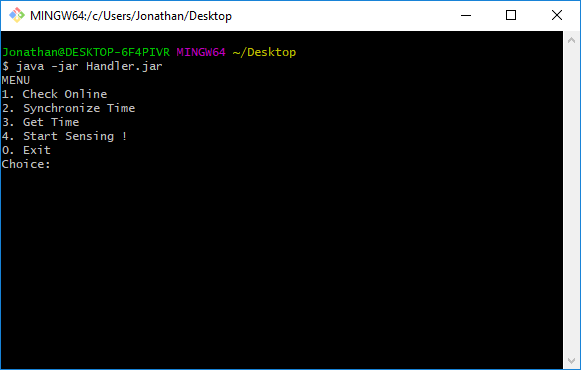
\includegraphics[scale=0.7]{menu_utama}
	\caption{Tampilan Utama Aplikasi}
	\label{fig:menu_utama}
\end{figure}
Fitur-fitur yang disediakan pada aplikasi ini adalah sebagai berikut:
\begin{enumerate}
    \item Check Online\\
    Fitur ini berfungsi untuk mengetahui node yang menyala pada satu jaringan. Untuk menjalankan fitur ini, pengguna harus memasukkan angka "1". Setelah pengguna telah memasukkan angka "1" maka sistem akan menampilkan node yang menyala seperti pada Gambar \ref{fig:menu_check_online}.
    \begin{figure}[H]
    	\centering
    	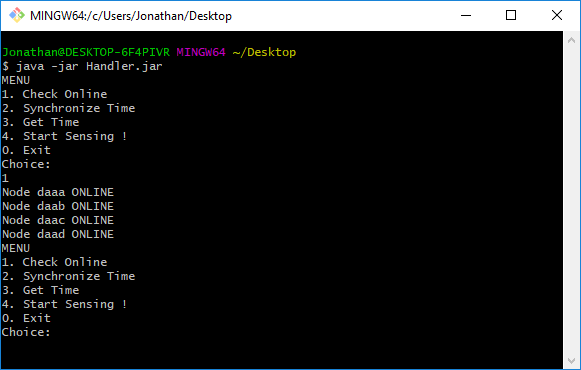
\includegraphics[scale=0.7]{menu_check_online}
    	\caption{Tampilan Check Online}
    	\label{fig:menu_check_online}
    \end{figure}
    \item Synchronize Time\\
    Fitur ini digunakan untuk melakukan sinkronisasi waktu setiap node sensor sesuai dengan waktu pada \textit{base station}. \textit{Base station} akan mengirimkan waktu yang didapat dari komputer pengguna kepada node sensor. Jika pengguna memasukkan angka "2" maka aplikasi akan menampilkan pesan "Done Synchronize" seperti pada Gambar \ref{fig:menu_synchronize_time}.
    \begin{figure}[H]
    	\centering
    	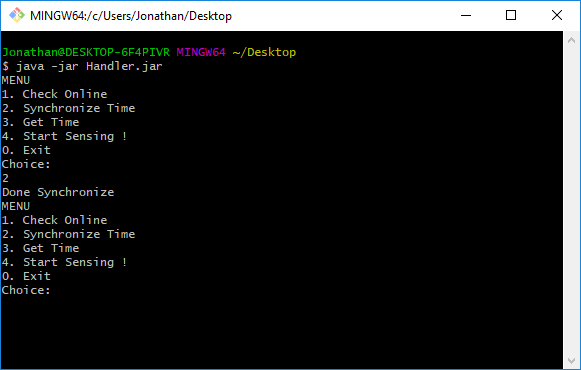
\includegraphics[scale=0.7]{menu_synchronize_time}
    	\caption{Tampilan Synchronize Time}
    	\label{fig:menu_synchronize_time}
    \end{figure}
    \item Get Time\\
    Fitur ini digunakan untuk mengetahui waktu dari setiap node sensor. Gambar \ref{fig:menu_get_time} adalah tampilan setelah pengguna memasukkan angka "3" untuk mengetahui waktu setiap node sensor.
    \begin{figure}[H]
    	\centering
    	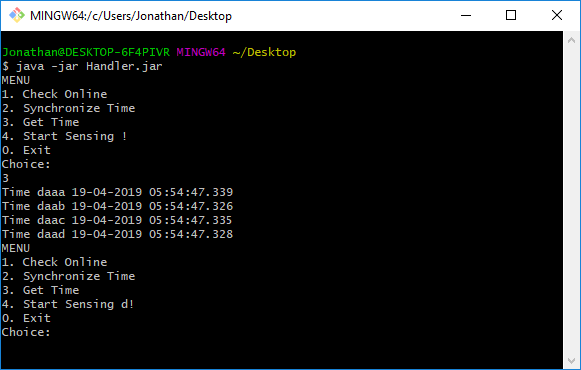
\includegraphics[scale=0.7]{menu_get_time}
    	\caption{Tampilan Get Time}
    	\label{fig:menu_get_time}
    \end{figure}
    \item Start Sensing\\
    Fitur ini digunakan sebagai fitur utama aplikasi yang telah dibangun. Aplikasi akan membuat node sensor melakukan \textit{sensing} dan hasilnya akan disimpan langsung ke dalam \textit{file text} untuk dilakukan analisis. 
    \item Exit\\
    Fitur ini digunakan untuk berhenti dan keluar dari aplikasi. Pengguna harus memasukkan angka "0" untuk berhenti dan keluar dari aplikasi ini seperti pada Gambar \ref{fig:menu_exit}.
    \begin{figure}[H]
    	\centering
    	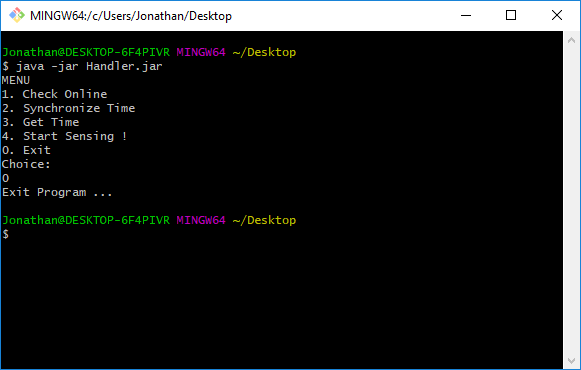
\includegraphics[scale=0.7]{menu_exit}
    	\caption{Tampilan Exit}
    	\label{fig:menu_exit}
    \end{figure}
    \item Kesalahan Masukkan.\\
    Masukkan yang tidak sesuai akan menampilkan pesan "Input Salah..." Gambar \ref{fig:salah_input_1} dan Gambar \ref{fig:salah_input_2} adalah tampilan saat ada kesalahan masukan.
    \begin{figure}[H]
    	\centering
    	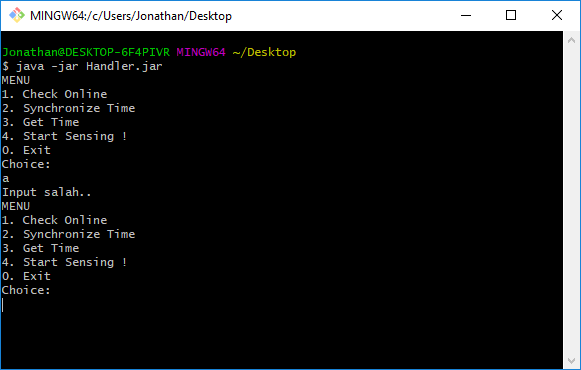
\includegraphics[scale=0.7]{salah_input_1}
    	\caption{Kesalahan Input 1}
    	\label{fig:salah_input_1}
    \end{figure}
    \begin{figure}[H]
    	\centering
    	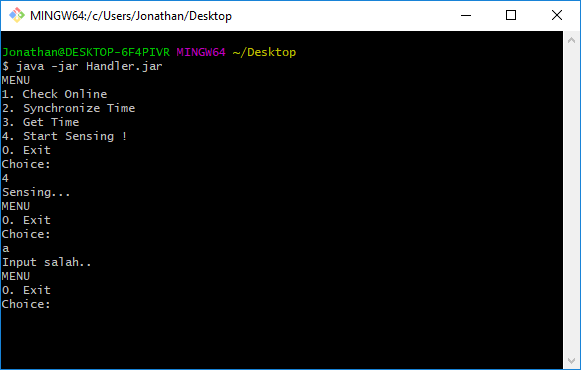
\includegraphics[scale=0.7]{salah_input_2}
    	\caption{Kesalahan Input 2}
    	\label{fig:salah_input_2}
    \end{figure}
\end{enumerate}

\subsection{Pengujian Eksperimental}
Pengujian eksperimental dilakukan di \textit{Rooftop} Gedung 10 Universitas Katholik Parahyangan sebagai ruang terbuka dan di dalam ruang tertutup. Arsitektur WSN yang digunakan saat pengujian adalah flat dengan \textit{single-hop} dan \textit{multi-hop}. Pengujian dilakukan dengan membandingkan data hasil \textit{sensing} aplikasi transfer yang \textit{reliable} dengan aplikasi transfer data yang tidak \textit{reliable}. Hal yang dibandingkan adalah \textit{sequence number} dan jumlah data yang \textit{loss}. 

Pengujian dilakukan dengan menggunakan 5 node sensor yang terdiri dari 1 node sensor sebagai \textit{base station} dan 4 node sensor untuk melakukan \textit{sensing}. Pengujian dilakukan sebanyak 1 kali untuk aplikasi transfer data \textit{reliable} dan 3 kali untuk aplikasi transfer data tidak \textit{reliable}. Pada setiap pengujian, diambil data \textit{sample} dengan sequence number dari 1 sampai 1000 setiap node sensor untuk dilihat berapa data yang \textit{loss}. 

Hasil dari setiap pengujian adalah tabel yang berisi jumlah data \textit{loss}. Tabel tersebut dibuat menjadi grafik untuk membandingkan jumlah \textit{loss} aplikasi transfer data \textit{reliable} dalam ruangan (IN R), \textit{reliable} pada ruang terbuka (OUT R), tidak \textit{reliable} dalam ruangan (IN NR), dan tidak \textit{reliable} pada ruang terbuka (OUT NR). 

\subsubsection{Single Hop}
\begin{figure}[H]
	\centering
	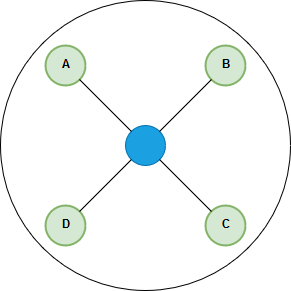
\includegraphics[scale=0.5]{singlehop}
	\caption{Arsitektur flat \textit{single-hop}}
	\label{fig:singlehop}
\end{figure}
Gambar \ref{fig:singlehop} adalah topologi yang penulis gunakan untuk melakukan pengujian pada arsitektur flat dengan \textit{single hop}. 
Hasil pengujian topologi \textit{single-hop} dapat dilihat pada Lampiran \ref{lamp:B}. Hasil yang didapat adalah tabel untuk setiap node sensor yang berisi jumlah data \textit{loss} pada setiap skenario. Gambar \ref{fig:grafik_single_hop_a} sampai Gambar \ref{fig:grafik_single_hop_d} adalah grafik hasil setiap node sensor pada topologi. \textit{single-hop}.
\begin{figure}[H]
	\centering
	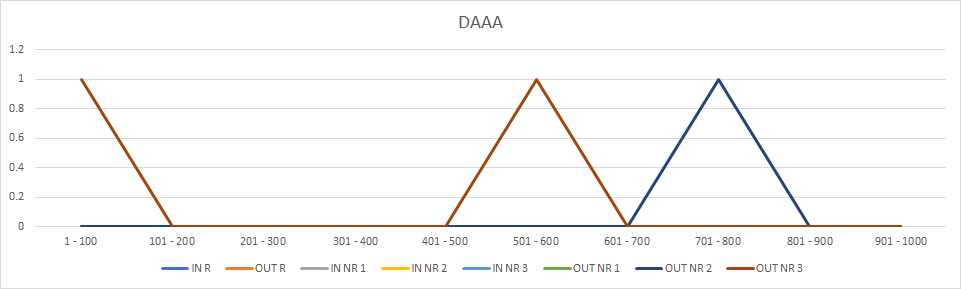
\includegraphics[scale=0.45]{grafik_single_hop_a}
	\caption{Grafik node DAAA pada single-hop}
	\label{fig:grafik_single_hop_a}
\end{figure}
\begin{figure}[H]
	\centering
	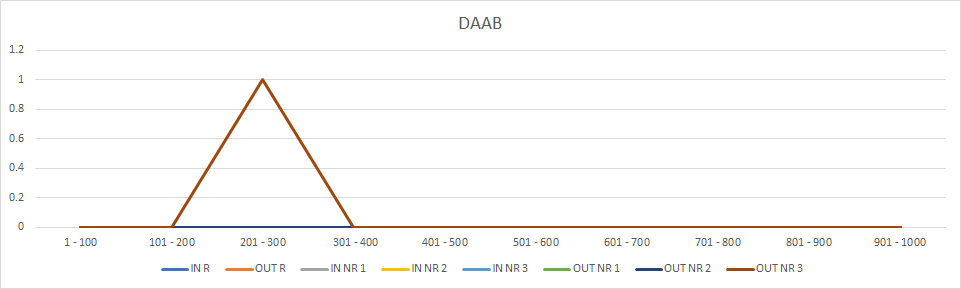
\includegraphics[scale=0.45]{grafik_single_hop_b}
	\caption{Grafik node DAAB pada single-hop}
	\label{fig:grafik_single_hop_b}
\end{figure}
\begin{figure}[H]
	\centering
	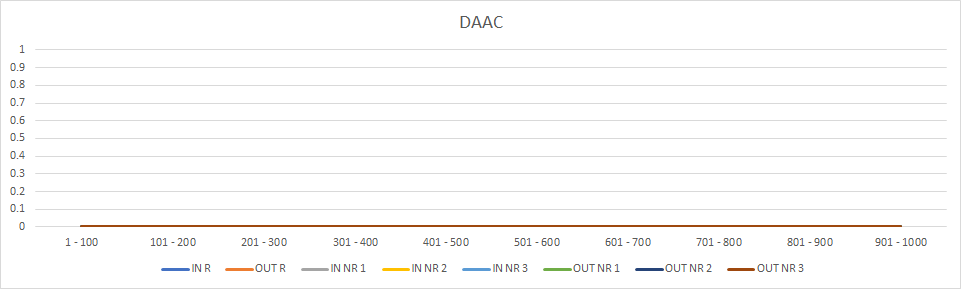
\includegraphics[scale=0.45]{grafik_single_hop_c}
	\caption{Grafik node DAAC pada single-hop}
	\label{fig:grafik_single_hop_c}
\end{figure}
\begin{figure}[H]
	\centering
	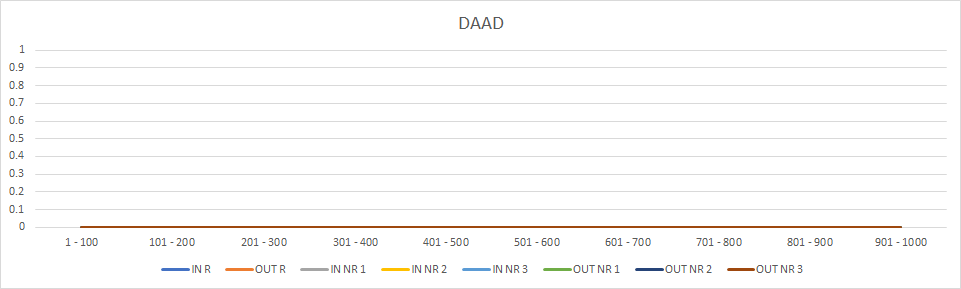
\includegraphics[scale=0.45]{grafik_single_hop_d}
	\caption{Grafik node DAAD pada single-hop}
	\label{fig:grafik_single_hop_d}
\end{figure}
Dari data yang diperoleh dapat dilihat bahwa pada topologi \textit{single-hop} untuk skenario dalam ruangan tidak terdapat \textit{loss} sedangkan untuk skenario ruang terbuka terdapat \textit{loss} hingga 2 data pada salah satu node sensor. Aplikasi transfer \textit{reliable} dan tidak \textit{reliable} tidak banyak perbedaan jumlah \textit{loss}. Hal ini karena pada \textit{layer network} sudah ditangani \textit{auto retry} jika tidak mendapatkan ACK.

\subsubsection{Multi Hop}

\begin{figure}[H]
	\centering
	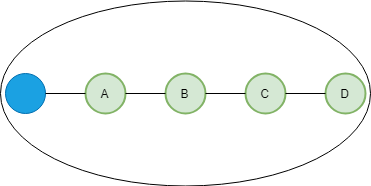
\includegraphics[scale=0.5]{1}
	\caption{Arsitektur flat \textit{multi-hop} tipe 1}
	\label{fig:1}
\end{figure}
Gambar \ref{fig:1} adalah topologi pertama yang penulis gunakan untuk melakukan pengujian pada arsitektur flat dengan \textit{multi-hop}. Hasil pengujian topologi \textit{multi-hop} tipe 1 dapat dilihat pada Lampiran \ref{lamp:C}. Hasil yang didapat adalah tabel setiap node sensor yang berisi jumlah data \textit{loss} pada setiap skenario. Gambar \ref{fig:grafik_multi_hop_1_a} sampai Gambar \ref{fig:grafik_multi_hop_1_d} adalah grafik hasil setiap node sensor pada topologi \textit{multi-hop} tipe 1.

\begin{figure}[H]
	\centering
	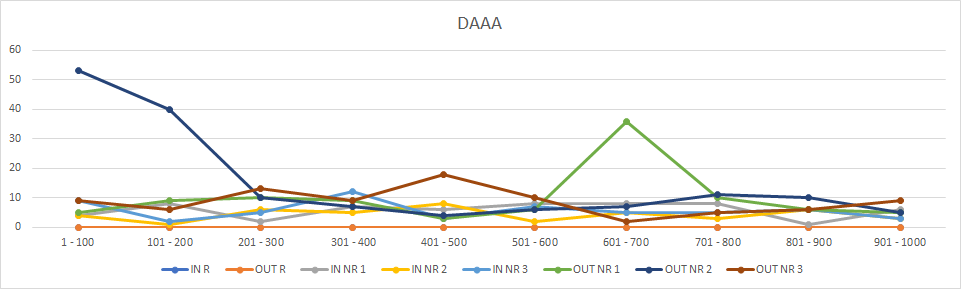
\includegraphics[scale=0.45]{grafik_multi_hop_1_a}
	\caption{Grafik node DAAA pada multi-hop tipe 1}
	\label{fig:grafik_multi_hop_1_a}
\end{figure}
\begin{figure}[H]
	\centering
	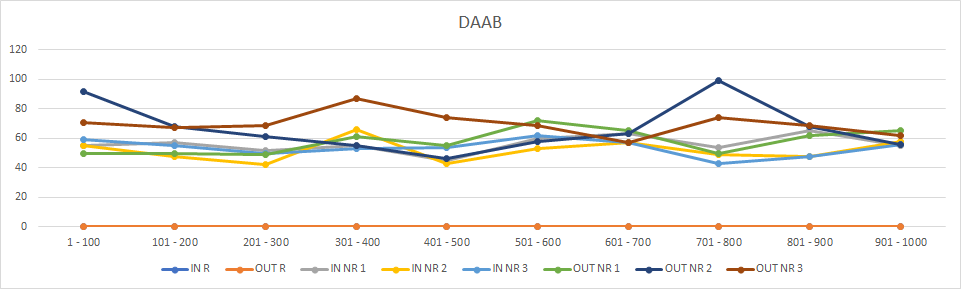
\includegraphics[scale=0.45]{grafik_multi_hop_1_b}
	\caption{Grafik node DAAB pada multi-hop tipe 1}
	\label{fig:grafik_multi_hop_1_b}
\end{figure}
\begin{figure}[H]
	\centering
	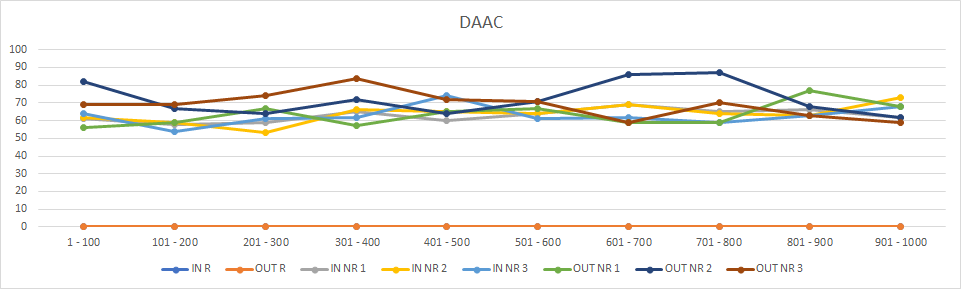
\includegraphics[scale=0.45]{grafik_multi_hop_1_c}
	\caption{Grafik node DAAC pada multi-hop tipe 1}
	\label{fig:grafik_multi_hop_1_c}
\end{figure}
\begin{figure}[H]
	\centering
	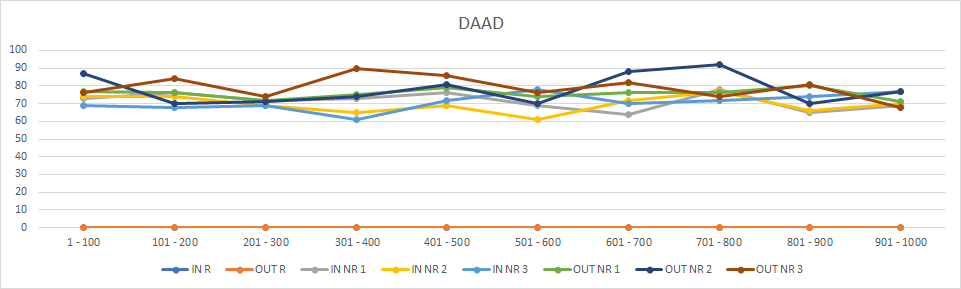
\includegraphics[scale=0.45]{grafik_multi_hop_1_d}
	\caption{Grafik node DAAD pada multi-hop tipe 1}
	\label{fig:grafik_multi_hop_1_d}
\end{figure}
Dari Gambar \ref{fig:grafik_multi_hop_1_a} sampai Gambar \ref{fig:grafik_multi_hop_1_d} didapat hasil aplikasi transfer yang tidak \textit{reliable} memiliki jumlah \textit{loss} yang berbeda-beda. Node DAAA mendapatkan \textit{loss} sekitar 10, node DAAB mendapatkan \textit{loss} sekitar 50 sampai 60, node DAAC mendapatkan \textit{loss} sekitar 55 sampai 70, dan node DAAD mendapatkan \textit{loss} lebih dari 70. Pada tipe ini semakin banyak hop yang harus dilalui sebuah data, maka semakin banyak juga \textit{loss} yang didapat. 

Sedangkan pada aplikasi transfer data yang \textit{reliable} jumlah \textit{loss} yang didapat adalah 0 di ruang terbuka dan di dalam ruangan. Aplikasi memastikan data sampai ke \textit{base station} dengan lengkap. 

\begin{figure}[H]
	\centering
	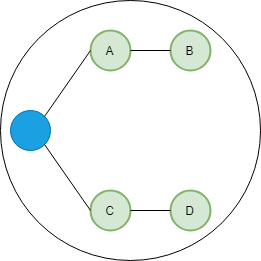
\includegraphics[scale=0.5]{2}
	\caption{Arsitektur flat \textit{multi-hop} tipe 2}
	\label{fig:2}
\end{figure}
Gambar \ref{fig:2} adalah topologi kedua yang penulis gunakan untuk melakukan pengujian pada arsitektur flat dengan \textit{multi-hop}. Hasil pengujian topologi \textit{multi-hop} tipe 2 dapat dilihat pada Lampiran \ref{lamp:D}. Hasil yang didapat adalah tabel untuk setiap node sensor yang berisi jumlah data \textit{loss} pada setiap skenario. Topologi \textit{multi-hop} tipe 2 ini memiliki perbedaan pada node yang terhubung langsung pada \textit{base station}. Hanya terdapat 2 node yang terhubung langsung dan node tersebut memiliki masing-masing satu node yang terhubung selain \textit{base station}. Gambar \ref{fig:grafik_multi_hop_2_a} sampai Gambar \ref{fig:grafik_multi_hop_2_d} adalah grafik hasil setiap node sensor pada topologi \textit{multi-hop} tipe 2.

\begin{figure}[H]
	\centering
	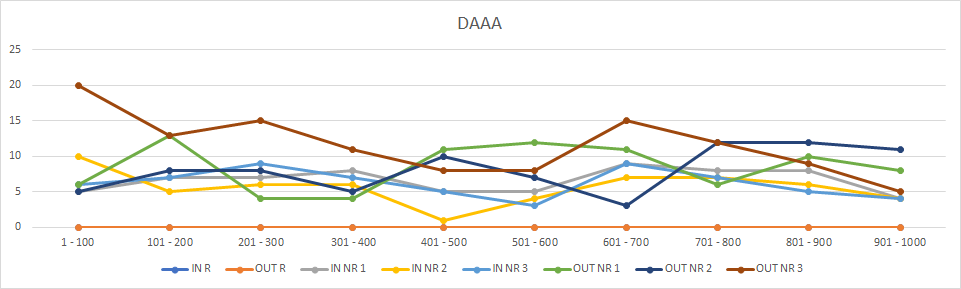
\includegraphics[scale=0.45]{grafik_multi_hop_2_a}
	\caption{Grafik node DAAA pada multi-hop tipe 2}
	\label{fig:grafik_multi_hop_2_a}
\end{figure}
\begin{figure}[H]
	\centering
	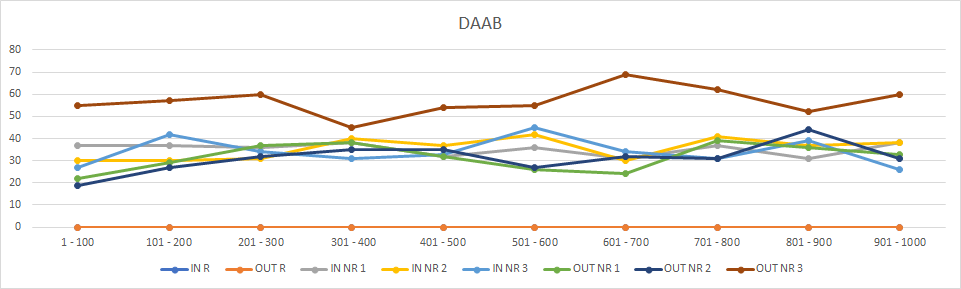
\includegraphics[scale=0.45]{grafik_multi_hop_2_b}
	\caption{Grafik node DAAB pada multi-hop tipe 2}
	\label{fig:grafik_multi_hop_2_b}
\end{figure}
\begin{figure}[H]
	\centering
	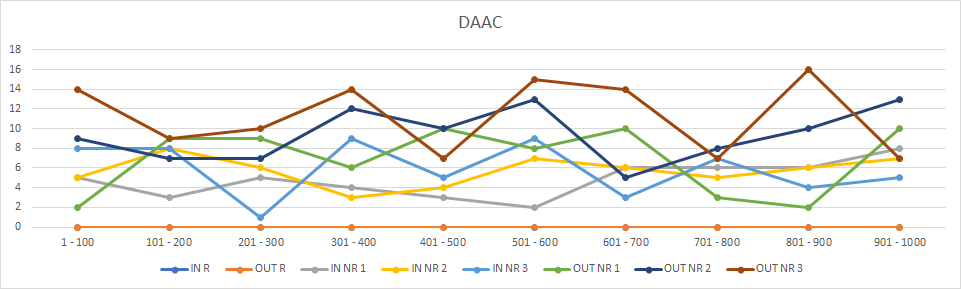
\includegraphics[scale=0.45]{grafik_multi_hop_2_c}
	\caption{Grafik node DAAC pada multi-hop tipe 2}
	\label{fig:grafik_multi_hop_2_c}
\end{figure}
\begin{figure}[H]
	\centering
	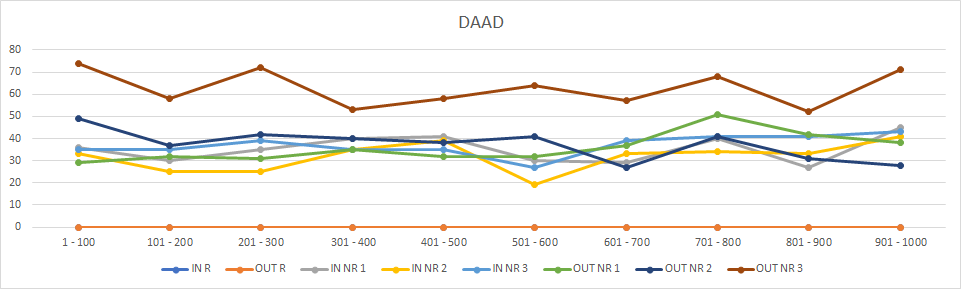
\includegraphics[scale=0.45]{grafik_multi_hop_2_d}
	\caption{Grafik node DAAD pada multi-hop tipe 2}
	\label{fig:grafik_multi_hop_2_d}
\end{figure}
Pada topologi \textit{multi-hop} tipe 2, node yang terhubung langsung pada \textit{base station} memiliki \textit{loss} yang lebih sedikit dibanding node lain. Node DAAA dan DAAB mendapatkan \textit{loss} dengan jumlah maksimal 20 \textit{loss} setiap 100 data. Sedangkan Node DAAC dan DAAD mendapatkan \textit{loss} dengan jumlah lebih dari 20 setiap 100 data. 

Pada pengujian aplikasi \textit{reliable} baik dalam ruangan maupun ruang terbuka, sama-sama memberikan hasil dengan jumlah \textit{loss} data 0.

\begin{figure}[H]
	\centering
	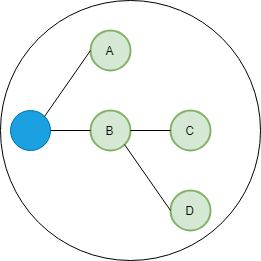
\includegraphics[scale=0.5]{3}
	\caption{Arsitektur flat \textit{multi-hop} tipe 3}
	\label{fig:3}
\end{figure}
Gambar \ref{fig:3} adalah topologi ketiga yang penulis gunakan untuk melakukan pengujian pada arsitektur flat dengan \textit{multi-hop}. Hasil pengujian topologi \textit{multi-hop} tipe 3 dapat dilihat pada Lampiran \ref{lamp:E}. 

\begin{figure}[H]
	\centering
	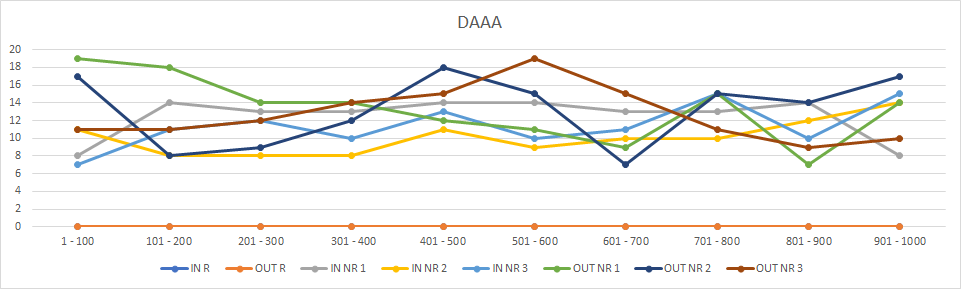
\includegraphics[scale=0.45]{grafik_multi_hop_3_a}
	\caption{Grafik node DAAA pada multi-hop tipe 3}
	\label{fig:grafik_multi_hop_3_a}
\end{figure}
\begin{figure}[H]
	\centering
	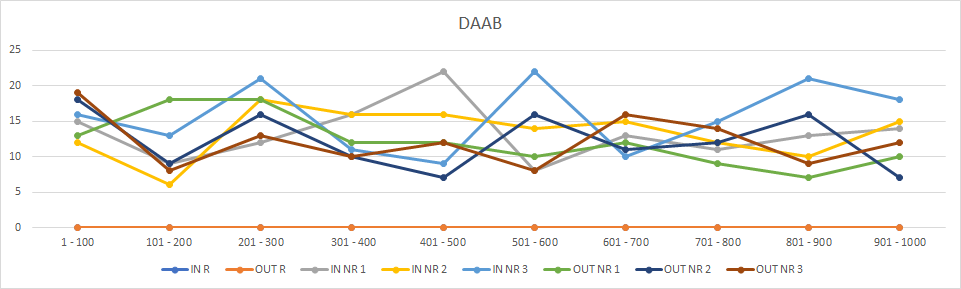
\includegraphics[scale=0.45]{grafik_multi_hop_3_b}
	\caption{Grafik node DAAB pada multi-hop tipe 3}
	\label{fig:grafik_multi_hop_3_b}
\end{figure}
\begin{figure}[H]
	\centering
	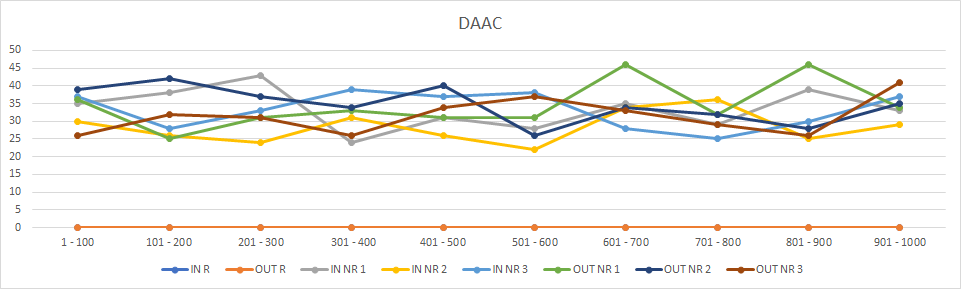
\includegraphics[scale=0.45]{grafik_multi_hop_3_c}
	\caption{Grafik node DAAC pada multi-hop tipe 3}
	\label{fig:grafik_multi_hop_3_c}
\end{figure}
\begin{figure}[H]
	\centering
	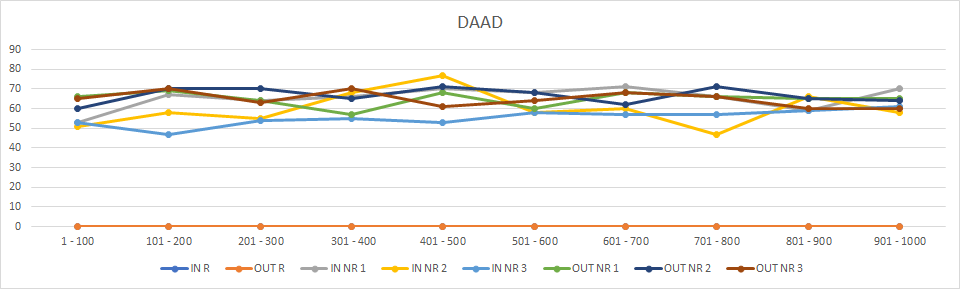
\includegraphics[scale=0.45]{grafik_multi_hop_3_d}
	\caption{Grafik node DAAD pada multi-hop tipe 3}
	\label{fig:grafik_multi_hop_3_d}
\end{figure}
Gambar \ref{fig:grafik_multi_hop_3_a} sampai Gambar \ref{fig:grafik_multi_hop_3_d} adalah grafik hasil setiap node sensor pada topologi \textit{multi-hop} tipe 3. Setiap node juga mendapatkan jumlah \textit{loss} yang beragam baik dari pengujian dalam ruangan maupun ruang terbuka. Pada aplikasi transfer data \textit{reliable}, node DAAA, DAAB, DAAC, dan DAAD tidak mendapatkan \textit{loss} pada setiap skenario.

Sedangkan pada aplikasi tidak \textit{reliable}, node DAAA mendapatkan jumlah \textit{loss} baik dalam ruangan maupun ruang terbuka adalah sekitar  5 sampai 20 setiap 100 data. Pada node DAAB, jumlah \textit{loss} adalah sekitar 5 sampai 20 setiap 100 data. Pada node DAAC mendapatkan jumlah \textit{loss} yang lebih banyak dibanding node DAAA dan DAAB yaitu sekitar 20 sampai 45 setiap 100 data. Pada node DAAD juga mendapatkan jumlah \textit{loss} yang lebih banyak dibanding node DAAA dan DAAB yaitu sekitar 50 sampai 70 setiap 100 data.

\begin{figure}[H]
	\centering
	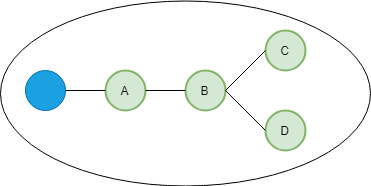
\includegraphics[scale=0.5]{4}
	\caption{Arsitektur flat \textit{multi-hop} tipe 4}
	\label{fig:4}
\end{figure}
Gambar \ref{fig:4} adalah topologi keempat yang penulis gunakan untuk melakukan pengujian pada arsitektur flat dengan \textit{multi-hop}. Hasil pengujian topologi \textit{multi-hop} tipe 4 dapat dilihat pada Lampiran \ref{lamp:F}. 

\begin{figure}[H]
	\centering
	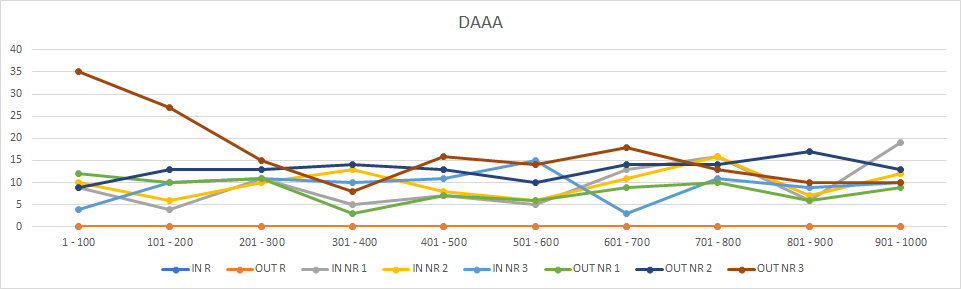
\includegraphics[scale=0.45]{grafik_multi_hop_4_a}
	\caption{Grafik node DAAA pada multi-hop tipe 4}
	\label{fig:grafik_multi_hop_4_a}
\end{figure}
\begin{figure}[H]
	\centering
	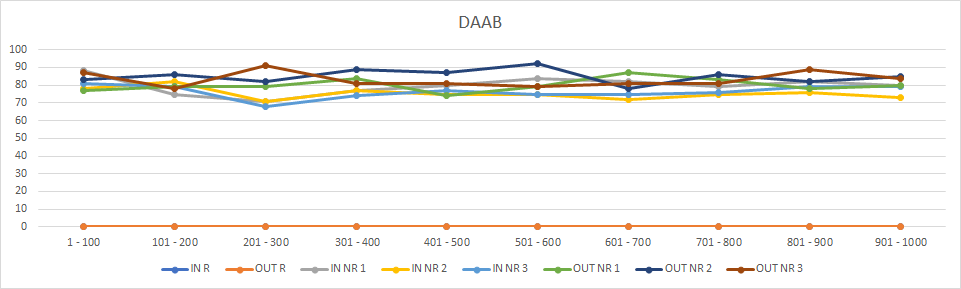
\includegraphics[scale=0.45]{grafik_multi_hop_4_b}
	\caption{Grafik node DAAB pada multi-hop tipe 4}
	\label{fig:grafik_multi_hop_4_b}
\end{figure}
\begin{figure}[H]
	\centering
	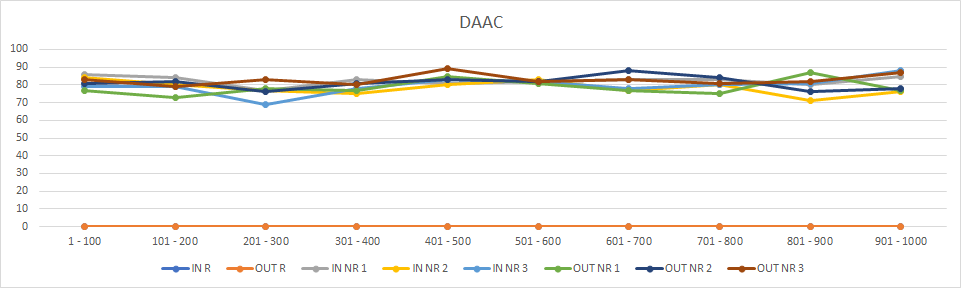
\includegraphics[scale=0.45]{grafik_multi_hop_4_c}
	\caption{Grafik node DAAC pada multi-hop tipe 4}
	\label{fig:grafik_multi_hop_4_c}
\end{figure}
\begin{figure}[H]
	\centering
	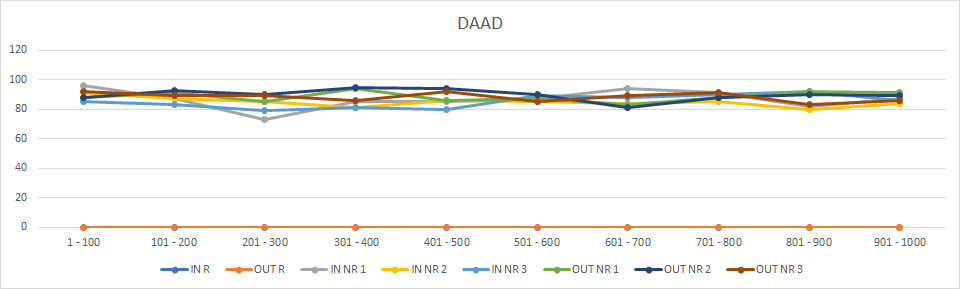
\includegraphics[scale=0.45]{grafik_multi_hop_4_d}
	\caption{Grafik node DAAD pada multi-hop tipe 4}
	\label{fig:grafik_multi_hop_4_d}
\end{figure}
Gambar \ref{fig:grafik_multi_hop_4_a} sampai Gambar \ref{fig:grafik_multi_hop_4_d} adalah grafik hasil setiap node sensor pada topologi \textit{multi-hop} tipe 4. Pada aplikasi transfer data \textit{reliable} node sensor DAAA, DAAB, DAAC, dan DAAD tidak mendapatkan \textit{loss} pada setiap skenario.

Pada node DAAA, jumlah \textit{loss} dari aplikasi tidak \textit{relibale} baik dalam ruangan maupun ruang terbuka adalah sekitar  5 sampai 20 setiap 100 data. Pada node DAAB, jumlah \textit{loss} adalah sekitar 70 sampai 90 setiap 100 data. Pada node DAAC mendapatkan jumlah \textit{loss} sekitar 70 sampai 95 setiap 100 data. Pada node DAAD mendapatkan jumlah \textit{loss} sekitar 80 sampai 100 setiap 100 data.

\begin{figure}[H]
	\centering
	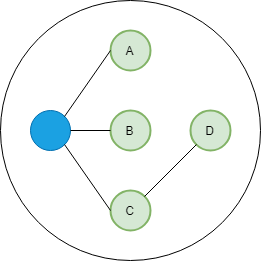
\includegraphics[scale=0.5]{5}
	\caption{Arsitektur flat \textit{multi-hop} tipe 5}
	\label{fig:5}
\end{figure}
Gambar \ref{fig:5} adalah topologi kelima yang penulis gunakan untuk melakukan pengujian pada arsitektur flat dengan \textit{multi-hop}. Hasil pengujian topologi \textit{multi-hop} tipe 5 dapat dilihat pada Lampiran \ref{lamp:G}. 

\begin{figure}[H]
	\centering
	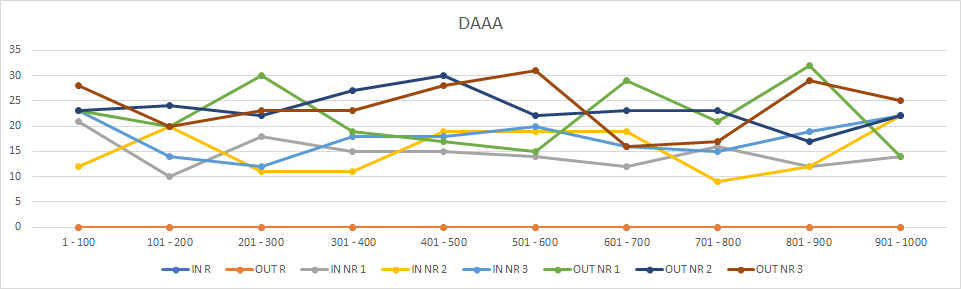
\includegraphics[scale=0.45]{grafik_multi_hop_5_a}
	\caption{Grafik node DAAA pada multi-hop tipe 5}
	\label{fig:grafik_multi_hop_5_a}
\end{figure}
\begin{figure}[H]
	\centering
	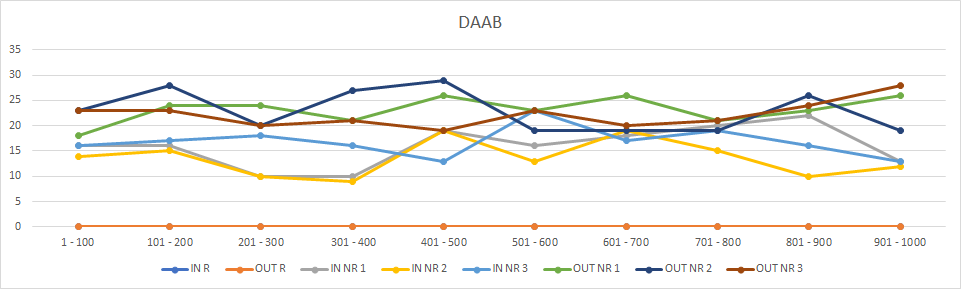
\includegraphics[scale=0.45]{grafik_multi_hop_5_b}
	\caption{Grafik node DAAB pada multi-hop tipe 5}
	\label{fig:grafik_multi_hop_5_b}
\end{figure}
\begin{figure}[H]
	\centering
	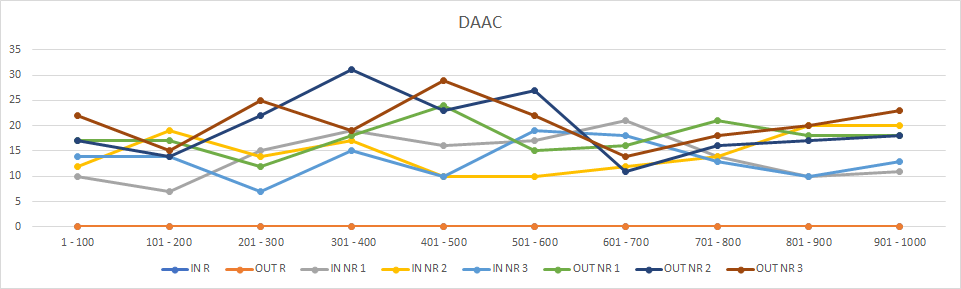
\includegraphics[scale=0.45]{grafik_multi_hop_5_c}
	\caption{Grafik node DAAC pada multi-hop tipe 5}
	\label{fig:grafik_multi_hop_5_c}
\end{figure}
\begin{figure}[H]
	\centering
	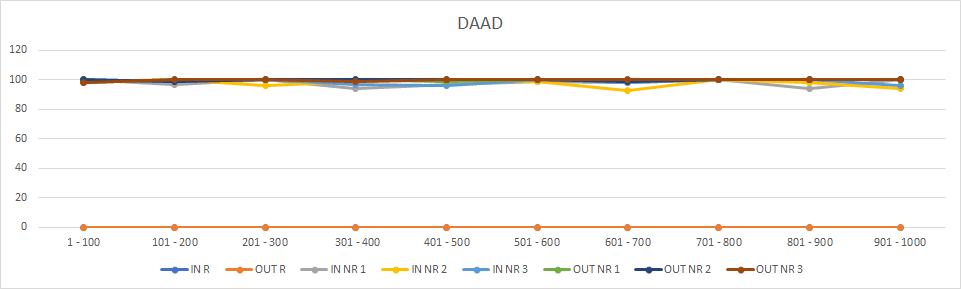
\includegraphics[scale=0.45]{grafik_multi_hop_5_d}
	\caption{Grafik node DAAD pada multi-hop tipe 5}
	\label{fig:grafik_multi_hop_5_d}
\end{figure}
Gambar \ref{fig:grafik_multi_hop_5_a} sampai Gambar \ref{fig:grafik_multi_hop_5_d} adalah grafik hasil setiap node sensor pada topologi \textit{multi-hop} tipe 5. Node DAAA pada aplikasi \textit{reliable} dan tidak \textit{reliable} dalam ruangan dan ruang terbuka mendapatkan \textit{loss} sekitar 10 sampai 35 data setiap 100 data. Pada node DAAB jumlah data \textit{loss} sekitar 10 sampai 30 data setiap 100 data. Node DAAC juga mendapatkan \textit{loss} data sekitar 5 sampai 30 data setiap 100 data. Node DAAD mendapatkan jumlah \textit{loss} sangat besar hampir semua data \textit{loss} pada setiap 100 data.

Sedangkan pada aplikasi transfer data \textit{reliable} setiap skenario, semua node sensor tidak mendapatkan \textit{loss}.

\subsection{Kesimpulan Hasil Eksperimen}
Dari setiap hasil eksperimen, kesimpulan yang dapat diambil oleh penulis yaitu dengan aplikasi transfer data \textit{reliable} yang telah dibuat dapat mengurangi jumlah \textit{loss} dari setiap skenario hingga 0 data \textit{loss}.

Aplikasi transfer data yang \textit{reliable} ini memiliki kelemahan sebagai konsekuensi yang harus diterima. Untuk mendapatkan 1000 data secara utuh dari setiap node sensor pada satu jaringan memerlukan waktu yang lebih lama dibandingkan aplikasi transfer data biasa. Hal ini disebabkan karena aplikasi ini menggunakan mekanisme ACK dan \textit{timer}. \textit{Timer} yang terjadi dapat lebih dari 1 kali yang membuat pengiriman data berikutnya menjadi tertunda. Tabel \ref{tab:waktu1} sampai Tabel \ref{tab:waktu3} perbandingan waktu yang diperlukan setiap node sensor mendapatkan data. SR adalah \textit{single-hop reliable}, SNR adalah \textit{single-hop} tidak \textit{reliable}, MH1R adalah \textit{multi-hop} tipe 1 \textit{reliable}, MH1NR adalah \textit{multi-hop} tipe 1 tidak \textit{reliable} dan seterusnya. "IN" adalah dalam ruangan dan "OUT" adalah ruang terbuka.

\begin{table}[H]
  \centering
  \caption{Perbandingan waktu yang diperlukan node sensor mengumpulkan data}
    \begin{tabular}{|p{1.3cm}|p{1.3cm}|p{1.3cm}|p{1.3cm}|p{1.3cm}|p{1.3cm}|p{1.3cm}|p{1.3cm}|p{1.3cm}|}
    \hline
        \multirow{2}{*}{Node}&\multicolumn{8}{|c|}{Waktu yang dibutuhkan (Menit)}\\
        \cline{2-9}
          & SR IN & SR OUT & SNR IN & SNR OUT & MH1R IN & MH1R OUT & MH1NR IN & MH1NR OUT \\
        \hline
        A     & 19.04 & 8.55  & 5.16  & 5.31  & 12.02 & 17.26 & 7.02  & 6.44 \\
    B     & 19.07 & 6.43  & 5.16  & 5.32  & 27.05 & 19.10  & 8.15  & 8.19 \\
    C     & 19.1  & 13.13 & 5.16  & 5.33  & 36.36 & 24.26 & 8.53  & 8.58 \\
    D     & 19.13 & 9.10   & 5.16  & 5.33  & 44.09 & 28.55 & 8.48  & 8.50 \\
    \hline
    \end{tabular}%
  \label{tab:waktu1}%
\end{table}%

\begin{table}[H]
  \centering
  \caption{Perbandingan waktu yang diperlukan node sensor mengumpulkan data}
    \begin{tabular}{|p{1.3cm}|p{1.3cm}|p{1.3cm}|p{1.3cm}|p{1.3cm}|p{1.3cm}|p{1.3cm}|p{1.3cm}|p{1.3cm}|}
    \hline
        \multirow{2}{*}{Node}&\multicolumn{8}{|c|}{Waktu yang dibutuhkan (Menit)}\\
        \cline{2-9}
          & MH2R IN & MH2R OUT & MH2NR IN & MH2NR OUT & MH3R IN & MH3R OUT & MH3NR IN & MH3NR OUT \\
        \hline
    A     & 8.40   & 8.47  & 6.46  & 6.54  & 11.24 & 7.17  & 4.04  & 3.32 \\
    B     & 13.30  & 14.32 & 6.46  & 4.49  & 14.54 & 19.19 & 9.15  & 8.48 \\
    C     & 8.38  & 8.09  & 6.46  & 6.49  & 21.06 & 19.19 & 9.11  & 8.47 \\
    D     & 14.54 & 14.56 & 6.43  & 4.47  & 22.28 & 19.19 & 9.09  & 6.55 \\
    \hline
    \end{tabular}%
  \label{tab:waktu2}%
\end{table}%

\begin{table}[H]
  \centering
  \caption{Perbandingan waktu yang diperlukan node sensor mengumpulkan data}
    \begin{tabular}{|p{1.3cm}|p{1.3cm}|p{1.3cm}|p{1.3cm}|p{1.3cm}|p{1.3cm}|p{1.3cm}|p{1.3cm}|p{1.3cm}|}
    \hline
        \multirow{2}{*}{Node}&\multicolumn{8}{|c|}{Waktu yang dibutuhkan (Menit)}\\
        \cline{2-9}
          & MH4R IN & MH4R OUT & MH4NR IN & MH4NR OUT & MH5R IN & MH5R OUT & MH5NR IN & MH5NR OUT \\
        \hline
    A     & 17.54 & 7.41  & 5.57  & 7.56  & 9.25  & 8.36  & 7.22  & 8.26 \\
    B     & 19.34 & 11.20  & 9.24  & 12.29 & 9.13  & 9.59  & 7.04  & 8.26 \\
    C     & 26.13 & 28.59 & 9.14  & 12.35 & 9.45  & 9.52  & 8.43  & 11.07 \\
    D     & 26.09 & 29.26 & 9     & 12.26 & 20.12 & 22.24 & 16.28 & 12.07 \\
    \hline
    \end{tabular}%
  \label{tab:waktu3}%
\end{table}%

Dari Tabel \ref{tab:waktu1} sampai Tabel \ref{tab:waktu3} dapat diambil kesimpulan bahwa aplikasi transfer data yang \textit{reliable} (R) memerlukan waktu yang lebih lama dibandingkan dengan aplikasi transfer data yang tidak \textit{reliable} (NR).

Aplikasi transfer data yang \textit{reliable} ini juga sangat boros dalam menggunakan sumber daya atau energi. Hal ini diakibatkan node sensor harus melakukan pengiriman ulang data yang \textit{loss} berkali-kali hingga node sensor tersebut mendapatkan ACK. Penggunaan energi paling besar pada WSN adalah saat melakukan transfer data. Jadi, untuk mencapai target jumlah data yang harus dikumpulkan diperlukan sumber daya yang banyak juga.

\section{Masalah yang Dihadapi pada Saat Implementasi}
Berikut adalah beberapa masalah yang dihadapi pada saat implementasi:
\begin{enumerate}
    \item Keterbatasan jumlah alat yang digunakan. Karena node sensor yang digunakan terbatas jadi harus digunakan bersama dengan mahasiswa lain yang menggunakan node sensor juga untuk skripsi mereka. 
    \item Node sensor ini sangat bergantung pada lingkungan sekitar. Jika terdapat penghalang sedikit saja maka akan memberikan hasil yang berbeda. Hal ini dikarenakan node sensor menggunakan gelombang radio sebagai media komunikasinya. Gelombang radio ini sangat mudah terintervensi oleh lingkungan sekitarnya seperti suhu, tembok, dan hujan.
    \item Saat pengujian node sensor dapat mati secara tiba-tiba. Node yang mati bisa bermacam-macam seperti node sensor untuk \textit{sensing}, node sensor perantara, maupun \textit{base station}. Hal ini diakibatkan karena ada masalah pada \textit{power} yang menghubungkan node sensor dengan baterai atau \textit{base staion} dengan \textit{port} komputer.
\end{enumerate}